\input templates/header
\title[DS - Epidemics 2]{\textbf{Distributed Algorithms}\\Epidemic Protocols: Beyond dissemination}
\usepackage{xmpmulti}

\begin{document}

\SetKwFor{METHOD}{function}{}{}
\SetKw{REAL}{real}

\newcommand{\ID}{\mathit{ID}}
\newcommand{\Request}{\textsc{request}}
\newcommand{\Reply}{\textsc{reply}}

\newcommand{\SelectNeighbor}{\alert{\mathsf{selectNeighbor}}}
\newcommand{\ExtractRequest}{\alert{\mathsf{prepareRequest}}}
\newcommand{\ExtractReply}{\alert{\mathsf{prepareReply}}}
\newcommand{\getPeer}{\alert{\mathsf{getPeer}}}
\newcommand{\MergeRequest}{\alert{\mathsf{mergeRequest}}}
\newcommand{\MergeReply}{\alert{\mathsf{mergeReply}}}
\newcommand{\Merge}{\alert{\mathsf{merge}}}

\newcommand{\getPair}{\mathsf{getPair}}
\newcommand{\View}{\mathit{view}}
\newcommand{\State}{\mathit{state}}
\newcommand{\Path}{\ell}

\newcommand{\Node}{\textsc{Node}\xspace}
\newcommand{\Random}{\textsf{random}\xspace}
\newcommand{\Extract}{\textsf{extract}\xspace}
\newcommand{\getTop}{\textsf{getTop}\xspace}

\newcommand{\MF}{\mathit{MF}}
\newcommand{\RF}{\mathit{RF}}
\newcommand{\AF}{\mathit{AF}}

\newcommand{\Freq}{\mathit{est}}


\newcommand{\SET}{\textbf{set}\xspace}
\newcommand{\LIST}{\textbf{list}\xspace}

\newcommand{\I}{I}

\newcommand{\F}{F}
\newcommand{\FR}{\hat{F}}

\newcommand{\Req}{\mathit{req}}
\newcommand{\Resp}{\mathit{rep}}

\newcommand{\Est}{\mathit{est}}

\newcommand{\FreqMF}{\textsc{FreqMF}\xspace}
\newcommand{\FreqAF}{\textsc{FreqAF}\xspace}
\newcommand{\FreqRF}{\textsc{FreqRF}\xspace}
\newcommand{\tput}{\textsc{tput}\xspace}


\global\long\def\N{N}
\global\long\def\M{M}
\global\long\def\m{m}

\global\long\def\K{k}
\global\long\def\S{s}
\global\long\def\D{d}


%-------------------------------------------------------------------------
{
\setbeamertemplate{footline}{} 
\setbeamertemplate{headline}{} 
\begin{frame}[noframenumbering]
	\titlepage
	\begin{center}
		\href{http://creativecommons.org/licenses/by-sa/4.0/}{This work is licensed under a Creative Commons Attribution-ShareAlike 4.0 International License.}
		
		\smallskip
		\includegraphics[width=1cm]{figs/cc.png}

	\bigskip
		{\tiny
			Acknowledgments: S. Voulgaris
		}
	\end{center}

	\invisible{
		\nobibliography*{references}
	}

\end{frame}
}






%%%%%%%%%%%%%%%%%%%%%%%%%%%%%%%%%%%%%%%%%%%%%%%%%%%%%%%%%%%%%%%%%%%%%%%%%%
\section{Peer Sampling}

\subsection{Introduction}

%-------------------------------------------------------------------------
\begin{frame}{System model}

\transdissolve

\BIL
\item A dynamic collection of distributed nodes that want to participate in a common epidemic protocol
\BI
\item Node may join / leave
\item Node may crash at any time
\EI
\item Communication:
\BI
\item To communicate with node $q$, node $p$ must know its address
\item Potentially high levels of message omissions
\EI
\EIL

\end{frame}

%-------------------------------------------------------------------------
\begin{frame}{Motivation}

\begin{columns}
\begin{column}{0.5\textwidth}
	
\structure{In the original paper}:\\
\BI
\item Nodes have \alert{full view} of the network
\item Each node periodically “gossips” with a random node, \textit{out of the whole set}
\EI
\bigskip
\structure{Why it was reasonable}:\\
\BI
\item (Almost) static network
\item Relatively small size 
\EI
\end{column}
\pause
\begin{column}{0.5\textwidth}
\structure{Currently}:\\
\BI
\item Nodes have a \alert{partial view} of the network
\item The partial view is \alert{dynamic}, reflecting nodes joining/leaving
\item Each node periodically gossips with a random node, \textit{out of its partial view}
\EI
\bigskip
\structure{What you get}:\\
\BI
\item Unlimited scalability
\item Capable to deal with churn
\EI
\end{column}
\end{columns}

\end{frame}
	

%-------------------------------------------------------------------------
\begin{frame}{Service specification}
	
\begin{block}{Peer sampling service}
\BI
\item \textbf{Input}: the distributed collection of nodes
\item \textbf{Output}: a method $\getPeer()$ that returns a peer as a
result of an independent uniform random sampling among the collection
\EI
\end{block}	
	
\bigskip
\structure{The idea}:\\
\BI
\item Nodes gossip with their neighbors about... other neighbors!
\item Old nodes are removed / new nodes are inserted
\item Random \alert{shuffling} of views
\EI
	
\end{frame}

%-------------------------------------------------------------------------
\begin{frame}{Service architecture}

% \begin{columns}
% \begin{column}{0.5\textwidth}
\BI
\item Each node has a view containing $C$ neighbors
\item Each node periodically contacts a neighbor 
\item They exchange their views
\EI
% \end{column}
% \begin{column}{0.5\textwidth}
% \end{column}
% \end{columns}

\bigskip
\begin{block}{The \alert{neighbor descriptor} of node $p$ contains}
\BI
\item The address needed to communicate with $p$
\item Timestamp information about the age of the descriptor
\item Additional information that may be needed by upper layers
\EI
\end{block}

\end{frame}

%-------------------------------------------------------------------------
\begin{frame}[shrink=5]{A generic algorithm}
	
\begin{Procedure}
\caption{Generic protocol executed by $p$:}

\UPON{initialization}{
  $\View \gets \textrm{descriptor(s) of nodes already in the system}$\;
}
\BlankLine
\REPEAT{every $\Delta$ time units}{
 $\Process\ q \gets \SelectNeighbor(\View)$\Comment*[f]{Select a random neighbor}\;
 $m \gets \ExtractRequest(\View, q)$\;
 \SEND $\langle \Request, m, p \rangle$ \TO $q$\;
}
\BlankLine
\UPON{\RECEIVE $\langle \Request, m, q \rangle$}{
 $m' \gets \ExtractReply(\View, q)$\;
 \SEND $\langle \Reply, m', p \rangle$ \TO $q$\;
 $\View \gets \Merge(\View, m, q)$\;
}
\BlankLine
\UPON{\RECEIVE $\langle \Reply, m, q \rangle$}{
 $\View \gets \Merge(\View, m, q)$\;
}
\end{Procedure}
	
\note{
\BIL
\item $\SelectNeighbor()$: select one of the neighbor contained in the view
\item $\ExtractRequest(\View, q)$, $\ExtractReply(\View, q)$: returns a subset of the descriptors contained in the local view; may add other descriptors (e.g. its own)
\item $\Merge(\View, m, q)$: returns a subset of the descriptors contained in the union of the local view and the received view
\EIL
}	
	
\end{frame}

%%%%%%%%%%%%%%%%%%%%%%%%%%%%%%%%%%%%%%%%%%%%%%%%%%%%%%%%%%%%%%%%%%%%%%%%%%
\subsection{\textsc{newscast}}

\begin{frame}{\textsc{newscast}}
	
\BI
\item $\SelectNeighbor()$\\
\BI
	\item Select one node at random from the local view
\EI
\item $\ExtractRequest(\View, q)$, $\ExtractReply(\View, q)$\\
\BI
	\item Returns the entire view + a local descriptor with a fresh timestamp
\EI
\item $\Merge(\View, m, q)$:\\
\BI
	\item Returns the $C$ freshest descriptors (w.r.t. timestamp) from the union of local view and message
\EI
\EI
	
\begin{Bib}
	\bibentry{newscast}
\end{Bib}	
	
\end{frame}

\begin{frame}{\textsc{newscast}}
	
\begin{overprint}
\onslide<1|handout:1>
\includegraphics[width=0.9\textwidth]{figs/11/1_newscast}
\onslide<2|handout:2>	
\includegraphics[width=0.9\textwidth]{figs/11/2_newscast}
\onslide<3|handout:3>	
\includegraphics[width=0.9\textwidth]{figs/11/3_newscast}
\onslide<4|handout:4>	
\includegraphics[width=0.9\textwidth]{figs/11/4_newscast}
\onslide<5|handout:5>	
\includegraphics[width=0.9\textwidth]{figs/11/5_newscast}
\onslide<6|handout:6>	
\includegraphics[width=0.9\textwidth]{figs/11/6_newscast}
\onslide<7|handout:7>	
\includegraphics[width=0.9\textwidth]{figs/11/7_newscast}
\onslide<8|handout:8>	
\includegraphics[width=0.9\textwidth]{figs/11/8_newscast}
\onslide<9|handout:9>	
\includegraphics[width=0.9\textwidth]{figs/11/9_newscast}
\onslide<10|handout:10>	
\includegraphics[width=0.9\textwidth]{figs/11/10_newscast}
\end{overprint}
\end{frame}

%%%%%%%%%%%%%%%%%%%%%%%%%%%%%%%%%%%%%%%%%%%%%%%%%%%%%%%%%%%%%%%%%%%%%%%%%%
\subsection{Cyclon}

\begin{frame}{Cyclon}
	
\BI
\item $\SelectNeighbor()$:
\BI
\item Select the oldest descriptor in the view
\EI
\item $\ExtractRequest(\View, q)$:
\BI
  \item Remove $t-1$ random neighbors from the local view
  \item Return the $t-1$ descriptors plus a fresh local one
\EI
\item $\ExtractReply(\View, q)$:
  \BI
  \item Remove and return $t$ fresh neighbors from the local view
  \EI
\item $\Merge(\View, m, q)$:
\BI
\item merge the local view and the message
\item remove $p$, keep freshes in case of duplicates
\item re-insert entries sent to $q$ if space permits
\EI
\EI
	
\begin{Bib}
	\bibentry{cyclon}
\end{Bib}	
	
\end{frame}


\begin{frame}{Cyclon}
	
\begin{overprint}
\onslide<1|handout:1>
\includegraphics[width=0.9\textwidth]{figs/11/1_cyclon}
\onslide<2|handout:2>	
\includegraphics[width=0.9\textwidth]{figs/11/2_cyclon}
\onslide<3|handout:3>	
\includegraphics[width=0.9\textwidth]{figs/11/3_cyclon}
\onslide<4|handout:4>	
\includegraphics[width=0.9\textwidth]{figs/11/4_cyclon}
\onslide<5|handout:5>	
\includegraphics[width=0.9\textwidth]{figs/11/5_cyclon}
\onslide<6|handout:6>	
\includegraphics[width=0.9\textwidth]{figs/11/6_cyclon}
\onslide<7|handout:7>	
\includegraphics[width=0.9\textwidth]{figs/11/7_cyclon}
\onslide<8|handout:8>	
\includegraphics[width=0.9\textwidth]{figs/11/8_cyclon}
\onslide<9|handout:9>	
\includegraphics[width=0.9\textwidth]{figs/11/9_cyclon}
\end{overprint}
\end{frame}


\begin{frame}{Experimental evaluation}

\begin{block}{Simulation parameters}
\BI
\item $N=100,000$ nodes
\item $C=20$ neighbors
\EI
\end{block}

\bigskip
\structure{We are measuring}:
\BI
\item Clustering coefficient
\item Average path length
\item Degree distribution
\item Robustness to catastrophic failures
\item Self-cleaning
\EI

\end{frame}

\begin{frame}{Brief recap}

\begin{definition}[Clustering coefficient]

The \alert{clustering coefficient} of graph $G$ is the average over the local 
  clustering coefficient of all nodes in the graph
  \[
     CC(G) = \frac{1}{N} \sum_{i \in V} \frac{2|E_i|}{|V_i|(|V_i|-1)}
  \]
\end{definition}

\bigskip
For epidemic diffusion:
\BI
\item high clustering coefficient means more redundant messages
\EI

\end{frame}

%-------------------------------------------------------------------------
\begin{frame}{Clustering coefficient}
	
\begin{center}
\includegraphics[width=0.8\textwidth]{figs/11/clustering}	
\end{center}
	
\note{
High clustering is bad for:
\BI
\item Flooding: It results in many redundant messages
\item Self-healing: Strongly connected cluster $\Rightarrow$ weakly connected to the rest of the network
\EI
}	

	
\end{frame}


\begin{frame}{Brief recap}

\begin{definition}[Average path length]
The \alert{average path length} of a connected graph $G=(V,E)$ is defined as:
\[
  \Path(G) = \frac{1}{|V|(|V|-1)} \sum_{i,j \in V, i \neq j} d(i,j)
\]
\end{definition}

\bigskip
For epidemic diffusion:
\BI
\item high average path length means a longer number of rounds to reach
  everybody else
\EI


\end{frame}

%-------------------------------------------------------------------------
\begin{frame}{Average path length}
	
\begin{center}
\includegraphics[width=0.8\textwidth]{figs/11/path}	
\end{center}

\note{
Indication of the time and cost to flood the network
}
	
\end{frame}


%-------------------------------------------------------------------------
\begin{frame}{Degree distribution}
	
\begin{center}
\includegraphics[width=0.8\textwidth]{figs/11/degree}	
\end{center}

\note{
Affects:
\BI
\item Robustness (shows weakly connected nodes)
\item Load balancing
\item Way epidemics spread
\EI


}


	
\end{frame}

%-------------------------------------------------------------------------
\begin{frame}{Robustness}
	
\begin{center}
\includegraphics[width=0.8\textwidth]{figs/11/robustness}	
\end{center}

\end{frame}

%-------------------------------------------------------------------------
\begin{frame}{Self-cleaning behavior}
	
\begin{center}
\includegraphics[width=0.8\textwidth]{figs/11/clean}	
\end{center}
	
\end{frame}

\subsection{Security}

\begin{frame}{Security}

\begin{columns}
\begin{column}{0.55\textwidth}
\begin{block}{Hub attack}
\BIL
\item Input: a set of colluding, malicious nodes 
\item How: they only gossip their IDs
\item Output: 
\BI
\item all views become “polluted”
\item non-malicious nodes are cut-off from each other
\item malicious nodes may leave the network, leaving the network disconnected with no way to recover
\EI
\EIL
\end{block}
\end{column}
\begin{column}{0.45\textwidth}
\begin{figure}
\includegraphics[width=0.7\textwidth]{figs/11/hub1}\\
\includegraphics[width=0.7\textwidth]{figs/11/hub2}	
\end{figure}
\end{column}
\end{columns}

\end{frame}

\begin{frame}{Secure peer sampling}
	
\begin{block}{Algorithm}
\BI
\item Maintain multiple independent views in each node
\item During a gossip exchange measure similarity of exchanged views
\item With probability equal to proportion of identical nodes in two views, reject the gossip and blacklist the node
\item Apply an aging policy to the black list
\item When supplying a random peer, select the current “best” view
\EI
\end{block}

\begin{Bib}
\bibentry{jesi}
\end{Bib}
	
\end{frame}

\begin{frame}{Secure peer sampling}

\begin{columns}
\begin{column}{0.55\textwidth}
\begin{figure}
\includegraphics[width=\textwidth]{figs/11/sps-architecture}
\end{figure}
\end{column}
\begin{column}{0.45\textwidth}
\begin{figure}
\includegraphics[width=\textwidth]{figs/11/sps-results}
\end{figure}

\BI
\item 1000 nodes
\item 20 malicious nodes
\EI

\end{column}
\end{columns}


\end{frame}



%%%%%%%%%%%%%%%%%%%%%%%%%%%%%%%%%%%%%%%%%%%%%%%%%%%%%%%%%%%%%%%%%%%%%%%%%%
\section{Topology construction}

%-------------------------------------------------------------------------
\begin{frame}{Introduction}

\begin{block}{Topology bootstrap}
Informal definition: \textit{building an overlay topology from the ground up as quickly and efficiently as possible}
\end{block}

\BIL
\item Do not confuse with node bootstrap
	\BI
	\item Placing a single node in the right place in the topology
	\EI
\item Do not confuse with topology maintenance
	\BI
	\item Stabilization (routing table cleanup)
	\item Can be used later to optimize the topology
	\EI
\EIL

\end{frame}

%-------------------------------------------------------------------------
\begin{frame}{State of the art}
	
\BIL
\item \alert{Current DHT protocols do not support bootstrapping}:\\
\BIL
\item They assume an already formed network
\item Even supposing the network exists, they work “unless a tremendous number of nodes joins the system” [Chord]
\item We could envision a “join orchestration approach”, but it would require a linear time
\EI
\EI

\pause
\begin{Bib}
\bibentry{tman}
\end{Bib}

\end{frame}

\subsection{T-Man}

%-------------------------------------------------------------------------
\begin{frame}{T-Man}
	
\BIL
\item T-man is a generic protocol for topology formation
\item Topologies are expressed through ranking functions:
	\BI
	\item “which are my preferred neighbors?”
	\EI
\EIL

\begin{columns}
\begin{column}{0.5\textwidth}
\BIL	
\item Examples
\BI
\item Rings, tori, trees, DHTs, etc.
\item Distributed sorting
\item Semantic proximity
\item Latency proximity 
\item Etc.	
\EI
\EIL
\end{column}	
\begin{column}{0.5\textwidth}
	\begin{figure}
	\includegraphics[width=0.6\textwidth]{figs/11/torus}
	\end{figure}
\end{column}	
\end{columns}	
\end{frame}

%-------------------------------------------------------------------------
\begin{frame}[shrink=5]{The T-Man algorithm}
	
\begin{Procedure}
\caption{Protocol executed by $p$:}

\UPON{initialization}{
  $\View \gets \textrm{a collection of random descriptors}$\;
}
\BlankLine
\REPEAT{every $\Delta$ time units}{
 $\Process\ q \gets \SelectNeighbor(\View)$\Comment*[f]{Select a neighbor}\;
 $m \gets \ExtractRequest(\View, q)$\;
 \SEND $\langle \Request, m, p \rangle$ \TO $q$\;
}
\BlankLine
\UPON{\RECEIVE $\langle \Request, m, q \rangle$}{
 $m' \gets \ExtractReply(\View, q)$\;
 \SEND $\langle \Reply, m', p \rangle$ \TO $q$\;
 $\View \gets \Merge(\View, m, q)$\;
}
\BlankLine
\UPON{\RECEIVE $\langle \Reply, m, q \rangle$}{
 $\View \gets \Merge(\View, m, q)$\;
}
\end{Procedure}

\end{frame}

%-------------------------------------------------------------------------
\begin{frame}{Node descriptors and ranking functions}
	
\begin{block}{Node descriptor}
\BI
\item IP address + timestamp, as in \textsc{newscast}/\textsc{cyclon}
\item One or more attributes of the node, used for ranking:
	\BI
	\item The ID of a node in a DHT; or
	\item A semantic description of the node; or
	\item The geographic location of the node
	\EI
\EI
\end{block}

\begin{block}{Ranking function}
\BI
\item A \alert{ranking function} $\mathit{rank}(U,p)$ ranks a collection $U$ of nodes based
on $p$'s order of preference.
\item Alternatively, a \alert{ranking function} $\mathit{rank}(U,p,r)$ returns $r$ nodes from
$U$ that are the most preferred by $p$.
\EI
\end{block}

\end{frame}

%-------------------------------------------------------------------------
\begin{frame}{Ranking functions}
	
\BIL
\item The ranking function may be based on a distance over a space
\BI
\item \alert{Space}: set of possible attribute values
\item \alert{Distance}: a metric $d(x,y)$ over the space 
\EI
\item Given a collection $U$ of nodes
\BI
\item rank them in increasing distance order, or
\item return the $r$ closest node based on the notion of distance
\EI
\EIL

\begin{columns}
\begin{column}{0.50\textwidth}
\begin{example}[Line/ring]
\BI
\item Space: $[0, 1)$
\item Distance over the line/ring:\\ 
  $d(a,b) = | a-b |$\\
  $d(a,b) = min \{ | a-b | , 1-|a-b| \}$
\EI
\end{example}
\end{column}
\begin{column}{0.45\textwidth}
\begin{example}[Grid or torus -- Manhattan Distance]
\BI
\item Space: $[0, 1) \cdot [0, 1)$
\item Distance: $d(a,b) = | a_x – b_x | + | a_y – b_y |$
\EI
\end{example}
\end{column}
\end{columns}
\end{frame}

\begin{frame}{How to express the ranking function}

\begin{columns}
\begin{column}{0.50\textwidth}
\structure{Generic line/ring}: returns
\BI
\item the $r$ nodes closest to $p$ w.r.t. the distance function
\invisible{\item the $r/2$ nodes “$\geq p$”, closest to $p$ w.r.t. the distance function
}
\EI
\begin{figure}
	\includegraphics[width=0.75\textwidth]{figs/11/unsorted-line}
\end{figure}
\end{column}
\begin{column}{0.50\textwidth}
\structure{Sorted line/ring}: returns
\BI
\item the $r/2$ nodes “$\geq p$”, closest to $p$ w.r.t. the distance function
\item the $r/2$ nodes “$\leq p$”, closest to $p$ w.r.t. the distance function
\EI

\begin{figure}
	\includegraphics[width=0.75\textwidth]{figs/11/sorted-line}
\end{figure}

\end{column}
\end{columns}

\end{frame}

%-------------------------------------------------------------------------
\begin{frame}{The T-Man algorithm}
	
\BI
\item $\SelectNeighbor()$
\BI
\item Select a random node from $\mathit{rank}(\View_p, p, r)$, i.e. from
the top-$r$ nodes in $p$'s local view as ranked by $p$
\EI
\item $\ExtractRequest(\View, q)$, $\ExtractReply(\View, q)$:
\BI
\item Returns $\mathit{rank}(\View_p, q, r)$, i.e. the top-$r$ nodes in $p$'s 
local view as ranked by $q$
\EI
\item $\Merge(\View, m, q)$:
\BI
\item merge the local view and the message
\EI
\EI
	
\end{frame}

\begin{frame}{T-Man: How it works}
	
\begin{overprint}
\onslide<1|handout:1>
\begin{figure}	
	\includegraphics[width=\textwidth]{figs/11/tman-1}
\end{figure}
\onslide<2|handout:2>
\begin{figure}	
	\includegraphics[width=\textwidth]{figs/11/tman-2}
\end{figure}
\end{overprint}

\end{frame}

\begin{frame}{T-Man: The movie!}
	
%\url{http://www.disi.unitn.it/~montreso/ds/handouts/ring-fingers-20.gif}

\begin{figure}
\multiinclude[graphics={width=0.60\textwidth},start=0,format=png]{figs/11/ring-fingers}
\end{figure}


\end{frame}


\begin{frame}{How to start and stop}
	
\structure{In the previous animation}:\\
\BIL
\item Nodes starts simultaneously
\item Convergence is measured globally
\EIL

\bigskip
\structure{In reality}:\\
\BIL
\item We must start the protocol at all nodes
\BI
\item Broadcasting, using the random topology obtained through a peer sampling services
\EI
\item We must stop the protocol
\BI
\item Local condition: when a node does not observe any view change for a predefined period, it stops
\item Idle: number of cycles without variations
\EI
\EIL

\end{frame}

%%%%%%%%%%%%%%%%%%%%%%%%%%%%%%%%%%%%%%%%%%%%%%%%%%%%%%%%%%%%%%%%%%%%%%%%%%
\subsection{Evaluation}

%-------------------------------------------------------------------------
\begin{frame}{Scalability, with different starting protocols}
	
\begin{figure}
	\includegraphics[width=0.80\textwidth]{figs/11/sort-size-ctime}
\end{figure}	
	
\end{frame}

%-------------------------------------------------------------------------
\begin{frame}{Bootstrap protocol: Starting and stopping}
	
\begin{figure}
	\includegraphics[width=0.80\textwidth]{figs/11/sort-active}
\end{figure}	
	
\end{frame}

%-------------------------------------------------------------------------
\begin{frame}{Stopping condition: different values for idle}
	
\begin{figure}
	\includegraphics[width=0.80\textwidth]{figs/11/sort-inactive-time}
\end{figure}	
	
\end{frame}

%-------------------------------------------------------------------------
\begin{frame}{Communication costs}
	
\begin{figure}
	\includegraphics[width=0.80\textwidth]{figs/11/sort-inactive-msg}
\end{figure}	
	
\end{frame}

%-------------------------------------------------------------------------
\begin{frame}{Parameter tuning: message size}
	
\begin{figure}
	\includegraphics[width=0.80\textwidth]{figs/11/sort-msgsize-time}
\end{figure}	
	
\end{frame}

%-------------------------------------------------------------------------
\begin{frame}{Robustness to failures}
	
\begin{figure}
	\includegraphics[width=0.80\textwidth]{figs/11/sort-crash}
\end{figure}	
	
\end{frame}

%-------------------------------------------------------------------------
\begin{frame}{Robustness to message losses}
	
\begin{figure}
	\includegraphics[width=0.80\textwidth]{figs/11/sort-loss-qual}
\end{figure}	
	
\end{frame}

%%%%%%%%%%%%%%%%%%%%%%%%%%%%%%%%%%%%%%%%%%%%%%%%%%%%%%%%%%%%%%%%%%%%%%%%%%
\subsection{T-Chord}

%-------------------------------------------------------------------------
\begin{frame}{T-Chord}
\animate<1-12>
	
\BIL	
\item The general idea:
	\BI
	\item Node descriptor contains node ID in a $[0..2^t)$ space
	\item Nodes are sorted over the ring defined by IDs
	\item Final output is the Chord ring
	\item As by-product, many other nodes are discovered
	\EI
\item Example:
	\BI
	\item $t=32$, $N=2^{14}$, $r=20$
	\EI
\EIL

\begin{figure}	
\multiinclude[graphics={width=0.80\textwidth},start=0,format=png]{figs/11/tchord}	
\end{figure}
	
\end{frame}

%-------------------------------------------------------------------------
\begin{frame}{T-Chord}

\BIL
\item Run T-Man until the ring is formed
\item Use the closest neighbors to select successors
\item Use the entire view to fill the finger table
	\BI
	\item For each node $p$:
	\item For each $i=0 \ldots m-1$ ($m$ number of bits)
	\item search in the local view \alert{the closest node} $q$ s.t.:
	\[
	q \in [(p + 2^i) \bmod 2^m, (p + 2^{i+1}-1) \bmod 2^m]
	\]
	\EI
\EIL

\end{frame}


%-------------------------------------------------------------------------
\begin{frame}{T-Chord-Prox}

\BIL
\item Run T-Man until the ring is formed
\item Use the closest neighbors to select successors
\item Use the entire view to fill the finger table
	\BI
	\item For each node $p$:
	\item For each $i=0 \ldots m-1$ ($m$ number of bits)
	\item search in the local view \alert{the closest node (in terms of latency)} $q$ s.t.:
	\[
	q \in [(p + 2^i) \bmod 2^m, (p + 2^{i+1}-1) \bmod 2^m]
	\]
	\EI
\EIL

\end{frame}

%-------------------------------------------------------------------------
\begin{frame}{Routing through T-Chord}

\begin{figure}
	\includegraphics[width=0.80\textwidth]{figs/11/chord-routing}
\end{figure}	


\end{frame}

%-------------------------------------------------------------------------
\begin{frame}{Robustness}

\begin{figure}
	\includegraphics[width=0.80\textwidth]{figs/11/chord-crash-fail}
\end{figure}	


\end{frame}

%%%%%%%%%%%%%%%%%%%%%%%%%%%%%%%%%%%%%%%%%%%%%%%%%%%%%%%%%%%%%%%%%%%%%%%%%%
\section{Aggregation}

%-------------------------------------------------------------------------
\begin{frame}{Aggregation}

\begin{definition}[Aggregation]
The collective name of a set of functions that provide statistical information about a system
\end{definition}

\BIL
\item Useful in large-scale distributed systems:
	\BI
	\item The average load of nodes in a computing grid
	\item The sum of free space in a distributed storage
	\item The total number of nodes in a P2P system
	\EI
\item Wanted: a decentralized, robust, proactive solution
\EIL

\begin{Bib}
	\bibentry{JMB05}
\end{Bib}

\end{frame}

%-------------------------------------------------------------------------
\begin{frame}[shrink=5]{A generic aggregation algorithm}
	
\begin{Procedure}
\caption{Protocol executed by $p$:}

\UPON{initialization}{
  $\State \gets \textrm{some initial state}$\;
}
\BlankLine
\REPEAT{every $\Delta$ time units}{
 $\Process\ q \gets \getPeer()$\Comment*[f]{Peer sampling service}\;
 $s_p \gets \ExtractRequest(\State, q)$\;
 \SEND $\langle \Request, s_p, p \rangle$ \TO $q$\;
}
\BlankLine
\UPON{\RECEIVE $\langle \Request, s_q, q \rangle$}{
 $s_p \gets \ExtractReply(\State, s_q, q)$\;
 \SEND $\langle \Reply, s_p, p \rangle$ \TO $q$\;
 $\State \gets \MergeRequest(\State, s_q, q)$\;
}
\BlankLine
\UPON{\RECEIVE $\langle \Reply, s_q, q \rangle$}{
 $\State \gets \MergeReply(\State, s_q, q)$\;
}
\end{Procedure}

\end{frame}

\subsection{Aggregation protocols}


\begin{frame}{Average aggregation}

\BIL
\item Local state maintained by nodes:
\BI
\item initialized with a real number representing the quantity to be averaged
\item contains the current estimate of the average
\EI 
\item  Function $\getPeer()$:
\BI
\item Based on peer sampling service
\item Returns a random peer from the entire collection of nodes
\EI
\item Function $\ExtractRequest(\State, q)$, $\ExtractReply(\State, s_q, q)$:
\BI
\item Returns $\State$
\EI
\item Function $\MergeRequest(\State, s_q, q)$, $\MergeReply(\State, s_q, q)$:
\BI
\item Returns $\frac{\State+s_q}{2}$
\EI
\EIL
\end{frame}

\begin{frame}{Example}
	
\begin{figure}
\begin{overprint}
\includegraphics<1|handout:1>[width=0.7\textwidth]{figs/11/aggregation1}
\includegraphics<2|handout:2>[width=0.7\textwidth]{figs/11/aggregation2}
\includegraphics<3|handout:3>[width=0.7\textwidth]{figs/11/aggregation3}
\includegraphics<4|handout:4>[width=0.7\textwidth]{figs/11/aggregation4}
\includegraphics<5|handout:5>[width=0.7\textwidth]{figs/11/aggregation5}
\includegraphics<6|handout:6>[width=0.7\textwidth]{figs/11/aggregation6}
\end{overprint}
\end{figure}

\end{frame}

%-------------------------------------------------------------------------
\begin{frame}{Average aggregation}

The exchange of messages is not atomic, so pairwise averaging is
better described in this way:
\BIL
\item Function $\ExtractRequest(\State, q)$
\BI
\item Returns $\State$
\EI
\item Function $\ExtractReply(\State, s_q, q)$:
\BI
\item Returns $\State-\frac{\State_q+s_q}{2}$
\EI
\item Function $\MergeRequest(\State, s_q, q)$:
\BI
\item Returns $\State - \left(\State-\frac{\State+s_q}{2} \right) = \frac{\State+s_q}{2}$
\EI
\item Function $\MergeReply(\State, d, q)$:
\BI
\item Returns $\State + d$
\EI
\EIL
\end{frame}



%-------------------------------------------------------------------------
\begin{frame}{Convergence}
	
\BIL
\item If the graph is connected, each node converges to the average of the original values
\item After each exchange:
	\BI
	\item Average does not change
	\item Variance is reduced
	\EI
\item Different from load balancing due to lack of constraints
\EIL

\end{frame}

%-------------------------------------------------------------------------
\begin{frame}{Convergence}
	
\begin{figure}
	\includegraphics[width=0.80\textwidth]{figs/11/average}
\end{figure}	
	
\end{frame}

%-------------------------------------------------------------------------
\begin{frame}{Other problems}

\BIL
\item \makebox[3.5cm][l]{\alert{Average}}	$\Merge(a,b)$ returns $(a+b)/2$
\item \makebox[3.5cm][l]{\alert{Geometric mean}}	$\Merge(a,b)$ returns $\sqrt{ab}$
\item \makebox[3.5cm][l]{\alert{Min/max}}	$\Merge(a,b)$ returns $\min(a,b)$ or $\max(a,b)$
\item \makebox[3.5cm][l]{\alert{Sum}}	Average $\cdot$ \alert{Count}
\item \makebox[3.5cm][l]{\alert{Product}}	Geometric $\cdot$ \alert{Count}
\item \makebox[3.5cm][l]{\alert{Variance}}	compute $\overline{a^2} - \overline{a}^2$
\EIL

\end{frame}

%-------------------------------------------------------------------------
\begin{frame}{Counting}
	
\begin{block}{Counting protocol}
\BI
\item Init: one node starts with $1$, all the others with $0$
\item Expected average: $1/N$
\EI
\end{block}

\smallskip
\BI
\item Problem: how to select that “one node”?
\item Concurrent instances of the counting protocol
\item Each instance is \textit{lead} by a different node
\item Messages are tagged with a unique identifier 
\item Nodes participate in all instances 
\item Each node acts as leader with probability $P=c/N_E$	
\EI
	
\end{frame}


\subsection{Analytical results}

%-------------------------------------------------------------------------
\begin{frame}{Questions}

\BIL
\item How fast is convergence on different topologies?
	\BI
	\item Analytical results for fully connected graphs: exponential convergence
	\item Random, \textsc{newscast} topologies: similar results
	\EI
\item Can we solve other problems
	\BI
	\item Counting, sum, variance estimation
	\EI
\item What are the effects of failures
	\BI
	\item Link failures: not critical
	\item Crashes/message omissions can ruin convergence
	\item But we have a solution for that
	\EI
\EIL

\end{frame}

%-------------------------------------------------------------------------
\begin{frame}{Analytical results}

\BI
\item Consider a “centralized translation” of the aggregation protocol
\item $N$ values to be aggregated are stored in vector $A$
\item An infinite number of rounds is executed 
\item At each round, the average operation is run on $N$ pairs of values
\EI

\smallskip
\begin{Procedure}
\caption{Aggregation}

\FOREVER{}{
  \For{$i \gets 1$ \TO $N$}{
    $(p,q) \gets \getPair()$\;
	$A[p], A[q] \gets (A[p]+A[q])/2$\;
  }
}
\end{Procedure}

\end{frame}

\begin{frame}{Some definitions}

\BIL
\item We measure the speed of convergence by measuring population mean
and variance at round $i$:
\[
\sigma_i^2 = \frac{1}{N} \sum_{k=1}^N (A_i[k] - \mu_i)^2
\quad \textrm{where} \quad
\mu_i = \frac{1}{N} \sum_{k=1}^N A_i[k] 
\]
\item Elementary variance reduction step:
\[
  \rho_i = {\sigma_{i+1}^2}/{\sigma^2_i} 
\]
\item Variable $\Phi_k$: the number of times that node $k$ has been selected from $\getPair()$
\EIL

\note{Unbiased estimator of the population variance:
\[
\sigma_i^2 = \frac{1}{N-1} \sum_{k=1}^N (A_i[k] - \mu_i)^2
\]
The term $N-1$ is called Bessel's correction
}

\end{frame}	

\begin{frame}{Analytical results}

\begin{theorem}[Convergence]
If
\BE
\item The indexes returned by each call to $\getPair()$ are uncorrelated;
\item the random variables $\Phi_k$ are identically distributed;
\item $\Phi$ is a random variable with this common distribution;
\item after $(p, q)$ is returned by $\getPair()$, the number of times $p$ and $q$ 
will be selected by the remaining calls to $\getPair()$ has identical distribution
\EE
then:
\[
  E[\sigma^2_{i+1}] = E[2^{-\Phi}] \sigma_i^2
\]	
\end{theorem}

\note{
  Explanation: $p$ and $q$ are selected in an independent way
}

\end{frame}

\begin{frame}{Analytical results}
\BIL
\item \alert{Optimal case}: $E(2^{-\Phi}) = E(2^{-2}) = 1/4$
\BI
\item $\getPair()$ implements perfect matching
\item no corresponding distributed protocol
\EI
\item \alert{Random case}: $E(2^{-\Phi}) = 1/e$
\BI
\item $\getPair()$ implements random global sampling
\item A local corresponding protocol exists
\EI
\item \alert{Aggregation protocol}: $E(2^{-\Phi}) = 1/(2\sqrt{e}) = 0.3032\ldots$ 
\BI
\item Scalability: results independent of $N$
\item Efficiency: convergence is very fast
\EI
\EIL

\end{frame}

%-------------------------------------------------------------------------
\begin{frame}{Convergence factor}

\begin{figure}
	\includegraphics[width=0.80\textwidth]{figs/11/rate-100000}
\end{figure}

\end{frame}

%-------------------------------------------------------------------------
\begin{frame}{Convergence factor}

\begin{figure}
	\includegraphics[width=0.80\textwidth]{figs/11/rate-av}
\end{figure}

\end{frame}

\subsection{Evaluation}

%-------------------------------------------------------------------------
\begin{frame}{Different topologies}
	
\BIL
\item Theoretical results are based on the assumption that the underlying overlay is  sufficiently random
\item What about other topologies?
\BI
\item Our aggregation scheme can be applied to generic connected topologies
\item Small-world, scale-free, newscast, random, complete
\item Convergence factor depends on randomness
\EI
\EIL
\end{frame}

%-------------------------------------------------------------------------
\begin{frame}{Different topologies}

\begin{figure}
	\includegraphics[width=0.80\textwidth]{figs/11/rate}
\end{figure}

\end{frame}

\begin{frame}{Different topologies}

%-------------------------------------------------------------------------
\begin{figure}
	\includegraphics[width=0.80\textwidth]{figs/11/reduction}
\end{figure}

\end{frame}


%-------------------------------------------------------------------------
\begin{frame}{Adaptivity}
	
\BIL
\item The generic protocol is not adaptive
	\BI
	\item Dynamism of the network
	\item Variability of values
	\EI
\item Periodical \alert{restarting} mechanism
	\BI
	\item  At each node:
		\BI
		\item The protocol is terminated	
		\item The current estimate is returned as the aggregation output
		\item The current values are used to re-initialize the estimates
		\item Aggregation starts again with fresh initial values
		\EI
	\EI
\EIL

\end{frame}

\begin{frame}{Dynamic membership}
	
\BIL
\item \alert{Termination} 
	\BI
	\item Run protocol for a predefined number of cycles $\lambda$
	\item $\lambda$ depends on:
		\BI
		\item required accuracy of the output
		\item the convergence factor that can be achieved
		\EI
	\EI
\item \alert{Restarting}
	\BI
	\item Divide run in consecutive epochs of length $\Delta$
	\item Start a new instance of the protocol in each epoch
	\EI
\item \alert{Node joining}
	\BI
	\item Receives from a node already in the network:
		\BI
		\item Next epoch identifier
		\item The time until the start of the next epoch
		\EI
	\item To guarantee convergence:
		\BI
		\item Joining node is not allowed to participate in the current epoch	
		\EI
	\EI
\EIL	
\end{frame}

\begin{frame}{Synchronization}
	
\BIL
\item The protocol described so far:
\BI
\item Assumes synchronized epochs and cycles
\item Requires synchronized clocks / communication
\EI
\item This is not realistic:
\BI
\item Clocks may drift
\item Communication incurs unpredictable delays
\EI
\item Complete synchronization is not needed
\BI
\item It is sufficient that the time between the first/ last node starting to participate in an epoch is bounded
\EI
\EIL

\end{frame}

\begin{frame}{Cost analysis}
	
\BIL
\item If the overlay is sufficiently random:
	\BI
	\item exchanges per round = $1 + \Phi$, where $\Phi$ has Poisson distribution with average $1$
	\EI
\item Round length $\delta$ defines trade-off between overhead and convergence
 	\BI
	\item $\delta = 1s$
	\item Overhead = $2 \cdot 2 \cdot (28+4) = 128$B/S
	\EI
\item N. of rounds $\lambda$ defines trade-off between accuracy and convergence:
	\BI
	\item $E(\sigma^2_\lambda )/E(\sigma_0^2) = \rho^\lambda$
	\item If $\epsilon$ the desired accuracy, then $\lambda \geq \log_\rho \epsilon$
	\EI
\EIL

\end{frame}


\begin{frame}{Evaluation}

\BIL	
\item Underlying topology is based on Newscast
\item The count protocol is used
	\BI
	\item More sensitive to failures
	\item Some parameters:
	\EI	
\item Some parameters:
	\BI
	\item Network size is $100.000$
	\item Partial view size in Newscast is $30$
	\item Epoch length is $30$ cycles
	\item Number of experiments is $50$
	\EI
\EIL
\end{frame}

%-------------------------------------------------------------------------
\begin{frame}{Sudden death}
	
\begin{figure}
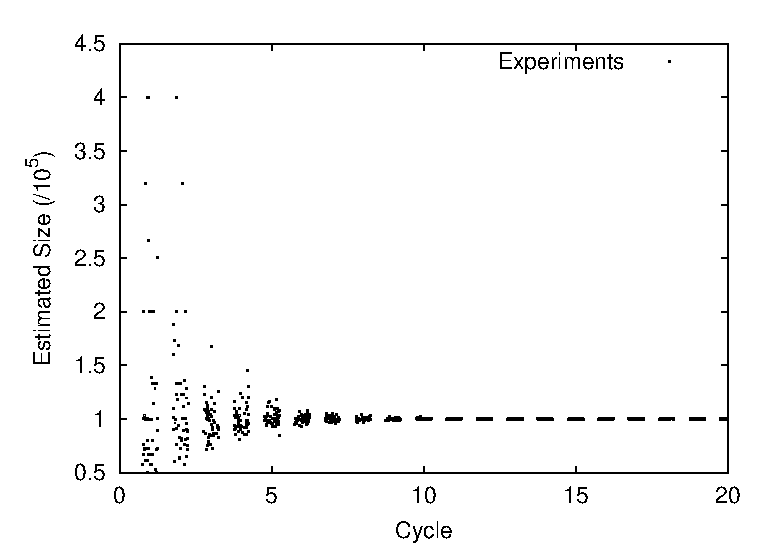
\includegraphics[width=0.80\textwidth]{figs/11/newscast-sudden-epoch}
\end{figure}

\note{Network size estimation where $50\%$ of the nodes crash suddenly.
The x-axis represents the cycle of an epoch at which the
``sudden death'' occurs.}
	
\end{frame}


%-------------------------------------------------------------------------
\begin{frame}{Churn}

\begin{figure}
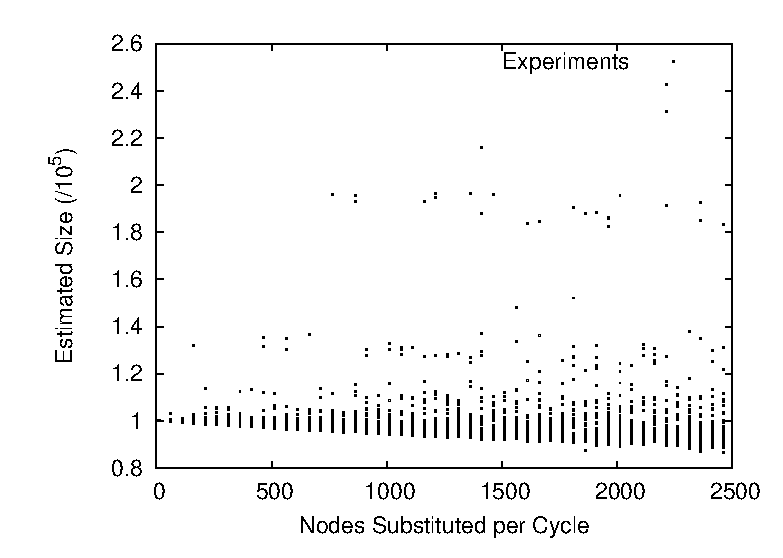
\includegraphics[width=0.80\textwidth]{figs/11/newscast-dynamic}
\end{figure}

\note{Network size estimation in a network of constant size subject to churn.
The x-axis is the churn rate which corresponds to the number of nodes that
crash at each cycle and are substituted by the same number of new nodes.}

\end{frame}

%-------------------------------------------------------------------------
\begin{frame}{Gnutella trace}

\begin{figure}
\includegraphics[width=0.80\textwidth]{figs/11/subtrace}
\end{figure}

\end{frame}

\note{Network size estimation in the presence of
churn according to a Gnutella trace.}

%-------------------------------------------------------------------------
\begin{frame}{Link failure probability}
	
\begin{figure}
\includegraphics[width=0.80\textwidth]{figs/11/newscast-fail-sym}
\end{figure}

\note{Convergence factor as a function of link failure probability.}
		
\end{frame}

%-------------------------------------------------------------------------
\begin{frame}{Message losses}

\begin{figure}
\includegraphics[width=0.80\textwidth]{figs/11/newscast-fail-asym}
\end{figure}

\note{Network size estimation as a function of lost messages.
The length of the bars illustrate
the distance between the minimal and
maximal estimated size over the set of nodes within a single experiment.}
		
\end{frame}

%-------------------------------------------------------------------------
\begin{frame}{Multiple executions}

\BIL
\item To improve accuracy in the case of failures:
	\BI
	\item Multiple concurrent instances of the protocol may be run
	\item Median value taken as result
	\EI
\item Simulations
	\BI
	\item Variable number of instances
	\item With node failures: 1000 nodes substituted per cycle
	\item With message omissions 20\% of messages lost
	\EI
\EIL
	
\end{frame}


%-------------------------------------------------------------------------
\begin{frame}{Multiple executions - churn}

\begin{figure}
\includegraphics[width=0.80\textwidth]{figs/11/multiple-crash-original}
\end{figure}

\note{Network size estimation with multiple instance. $1000$ nodes crash at the beginning of each cycle.
The length of the bars correspond to the distance between the minimal and
maximal estimates over the set of all nodes within a single experiment.}

\end{frame}

%-------------------------------------------------------------------------
\begin{frame}{Multiple executions - churn}
\begin{figure}
\includegraphics[width=0.80\textwidth]{figs/11/multiple-omission-original}
\end{figure}

\note{Network size estimation as a function of
concurrent protocol instances.   20\% of messages are lost.
The length of the bars correspond to the distance between the minimal and
maximal estimates over the set of all nodes within a single experiment.}

\end{frame}

%-------------------------------------------------------------------------
\begin{frame}{Planet-lab}

\BI
\item PlanetLab is a global research network that supports the development of new network services
\item PlanetLab currently consists of 1075 nodes at 525 sites
\EI

\begin{figure}
\includegraphics[width=0.80\textwidth]{figs/11/planetlab}
\end{figure}

\end{frame}


%-------------------------------------------------------------------------
\begin{frame}{Planet-lab}
\begin{figure}
\includegraphics[width=0.80\textwidth]{figs/11/planet}
\end{figure}

\note{The estimated size and the actual size
of a network oscillating between 2500 and 6000 nodes (approximately). Standard
deviation of estimated size is displayed using vertical bars.}

\end{frame}

\subsection{Most frequent items}

\begin{frame}{Most frequent items}

\begin{block}{System model}

\BI
\item A collection $\Process$ of nodes of size $N=|\Process|$
\item Each node $p \in \Process$ stores a local multiset $I_p$ of items taken
from a universe $\cal I$ of size $m=|\cal I|$
\EI
\end{block}

\begin{block}{Problem statement}
Identify the $\K$ \alert{most frequent items}, i.e. the $\K$ distinct items
that appear more frequently in the distributed multiset given by 
$I = \bigcup_{p \in \Process} I_p$
\end{block}

\begin{Bib}
	\bibentry{computing12}
\end{Bib}

\end{frame}


\begin{frame}{Formal model}

\begin{block}{Global frequency}
\begin{align*}
\textrm{\alert{Global absolute frequency}}: \qquad& \F(i) = \sum_{p \in \Process} \F_p(i) \\
\textrm{\alert{Global relative frequency}}: \qquad& \FR(i) = \F(i)/\M
\end{align*}
Note: $M = |I|$
\end{block}

\begin{block}{Most frequent items}
Let $j$ be the $\K$-th item in the sequence of all items ordered by decreasing
global frequency. We want to identify the top-$\K$ most frequent items:
\[
  \MF = \{ i : \F(i) \geq \F(j) \}
\]
\end{block}


\end{frame}

\begin{frame}{Formal model}

\begin{block}{Absolutely frequent items}
To identify \alert{absolutely frequent} items ($\AF$) whose
global absolute frequency is larger than the absolute threshold $f$:
\[
  \AF = \{ i : \F(i) \geq f \}
\]
\end{block}

\medskip
\begin{block}{Relatively frequent items}
To identify \alert{relatively frequent} items ($\RF$) whose
global relative frequency is larger than the relative threshold $\phi$:
\[
  \RF = \{ i : \FR(i) \geq \phi \}
\]
\end{block}

\end{frame}

\begin{frame}{Solution}
	
\begin{block}{Naive protocol}
\BI
\item Compute the \alert{average global frequency} $\F(i)/N$ of all items
\item Sort items by decreasing frequency
\item Identify the item $j$ ranked $\K$-th in such ordered sequence
\item Return the items whose average frequency is larger or equal
than $\F(j)/N$
\EI
\end{block}
	
\end{frame}

\begin{frame}{\FreqMF protocol (1)}
	\begin{Procedure}

\caption{\FreqMF algorithm executed by node $p$}

\UPON{initialization}{
  $\Map\ \Est_p \gets \NEW\ \Map()$\;
  \ForEach{$i \in \I_p$}{
    $\Est_p[i] \gets \F_p(i)$\;
  }
}
\BlankLine
\METHOD{\getTop($\K$)}{
  \Return\ $\Extract(\Est_p, \K)$\;
}
\BlankLine
\REPEAT{every $\Delta$ time units}{
  $\Node\ q \gets \Random(\Process)$\;
  \SEND $\langle \Request, \Extract(\Est_p, \S) \rangle$ \TO $q$\;
}
\end{Procedure}

\end{frame}

\begin{frame}{\FreqMF protocol (2)}
	\begin{Procedure}

\caption{\FreqMF algorithm executed by node $p$}

\UPON{$\RECEIVE \langle \Request, \Req_q \rangle$ \FROM $q$}{
  $\Map\ \Resp_p \gets \NEW\ \Map()$\;
  \ForEach{$i \in \Req_q$}{
    $\REAL\ \delta_i \gets \frac{1}{2}(\Req_q[i]-\Est_p[i])$\;
    $\Est_p[i] \gets \Est_p[i]+ \delta_i$\;
    $\Resp_p[i] \gets \delta_i$\;
  }
  \SEND $\langle \Reply, \Resp_p \rangle $ \TO $q$\;
}
\BlankLine
\UPON{$\RECEIVE \langle \Reply, \Resp_q \rangle$}{
  \ForEach{$i \in \Resp_q$}{
    $\Est_p[i] \gets \Est_p[i]-\Resp_q[i]$\;
  }
}
\end{Procedure}

\end{frame}

\begin{frame}{\FreqAF and \FreqRF protocols}
	
\BI
\item How can you implement the \FreqAF protocol?
\item How can you implement the \FreqRF protocol?
\EI

\end{frame}

\begin{frame}{\FreqMF evaluation}

\begin{figure}
\includegraphics[width=0.9\textwidth]{figs/11/msgsize.pdf}
\end{figure}

\end{frame}

\begin{frame}{\FreqMF evaluation}

\begin{figure}
\includegraphics[width=0.9\textwidth]{figs/11/msgoverhead.pdf}
\end{figure}

\end{frame}

\begin{frame}{\FreqMF evaluation}

\begin{figure}
\includegraphics[width=0.9\textwidth]{figs/11/msgstorage.pdf}
\end{figure}

\end{frame}

\begin{frame}{\FreqMF evaluation}

\begin{figure}
\includegraphics[width=0.9\textwidth]{figs/11/msgratio.pdf}
\end{figure}

\end{frame}


%%%%%%%%%%%%%%%%%%%%%%%%%%%%%%%%%%%%%%%%%%%%%%%%%%%%%%%%%%%%%%%%%%%%%%%%%%
\section{Bibliography}

%-------------------------------------------------------------------------
\begin{frame}{Reading material}

{\footnotesize
\BIL
\item \bibentry{peersampling}
\item \bibentry{JMB05}
\EIL
}

\invisible{{\tiny
\bibliographystyle{abbrv}
\bibliography{references} 
}}

\end{frame}

\end{document}